\chapter{Bolas de fuego, sistemas de referencia y cuadrivectores}

Comenzamos con una pregunta que quedó pendiente de la discusión sobre colisiones de alta energía. La colisión de dos núcleos pesados crea un objeto que cambia violentamente, no un agujero negro astronómico tranquilo. ¿Qué puede significar, entonces, describir la colisión mediante un horizonte? La respuesta pasa por una imagen pentadimensional de la materia fuertemente acoplada y por una serie de preguntas prácticas sobre los aceleradores, para volver finalmente a la geometría de la relatividad especial. Al final, la velocidad y el momento se habrán convertido en cuadrivectores, y la energía ocupará su lugar junto a las tres componentes del momento.

\section{Una bola de fuego en una quinta dimensión}

\begin{classroomqa}\audiencequestion{El objeto producido en la colisión es inestable y cambia de forma. ¿Cómo se puede llamar agujero negro a un objeto tan complicado?}\lecturerresponse{Imaginemos una quinta dirección espacial que se extiende entre un suelo y un techo. La gravedad en esa dirección atrae las excitaciones hacia el suelo. La colisión deposita allí una masa de energía caliente; esta se expande y cambia de forma, pero aun así puede tener horizonte, temperatura y entropía.}\end{classroomqa}

Imaginemos partículas o, de forma más gráfica, pequeñas cuerdas que se mueven en este mundo pentadimensional. Las excitaciones que caen hacia el suelo aparecen en cuatro dimensiones como hadrones: protones, neutrones, mesones y otros objetos compuestos extendidos. Las excitaciones situadas cerca del techo parecen más elementales. Por tanto, la posición vertical es una forma geométrica de codificar la escala: el suelo representa el régimen hadrónico de grandes distancias, mientras que el techo representa los grados de libertad de distancias cortas.

Cuando chocan dos hadrones, dos objetos cerca del suelo se golpean y producen una gran salpicadura de energía. El resultado no es un cuerpo rígido. Es una masa caliente con horizonte, una especie de charco en el campo gravitatorio pentadimensional. No es un agujero negro astronómico en el espacio ordinario de cuatro dimensiones ni un agujero negro a escala de Planck situado junto al techo. Es la descripción gravitatoria de la bola de fuego fuertemente interactuante cerca del suelo.

A alta energía, los núcleos incidentes se contraen por Lorentz hasta convertirse en panqueques delgados. Chocan, depositan su energía en una región pequeña y producen un fluido que se expande hacia el equilibrio. Su baja viscosidad fue una de las características sorprendentes del plasma de quarks--gluones. En la descripción pentadimensional, la misma evolución es la relajación de un horizonte distorsionado.

\begin{figure}[H]\centering
\includegraphics[width=0.82\textwidth]{lecture_05_figure_01.png}\caption{La imagen del suelo y el techo para la quinta dimensión. Tras la colisión, la masa central con horizonte se expande a lo largo del suelo.}\lectureframe{00:04:22}\end{figure}

Un horizonte no dura para siempre. La radiación de Hawking se lleva energía y, en la descripción tetradimensional, esa radiación es la lluvia de hadrones ordinarios que emerge de la colisión. En este lenguaje, los miles de trazas de un suceso registrado por un detector son las partículas que se desprendieron por evaporación del agujero negro dual.

\subsection{¿Es real la dimensión extra?}

\begin{classroomqa}\audiencequestion{¿Es la quinta dimensión una dimensión espacial? ¿La línea dibujada entre el suelo y el techo se extiende literalmente en esa dirección?}\lecturerresponse{Sí. Es espacial, y la superficie dibujada en esa geometría pentadimensional es un horizonte. Si se llama ``real'' a esa dirección adicional o se la considera una descripción matemática equivalente es una cuestión más profunda.}\end{classroomqa}

La afirmación útil no es que la gravedad sustituya a la cromodinámica cuántica. Más bien, dos lenguajes pueden describir la misma física. En el lenguaje tetradimensional hay una bola de fuego caliente de quarks y gluones, sin un campo gravitatorio ordinario. En el lenguaje pentadimensional hay gravedad y un horizonte. Si la correspondencia es correcta, un cálculo genuino de QCD y el cálculo gravitatorio dual deben concordar allí donde ambos puedan realizarse.

\begin{classroomqa}\audiencequestion{La QCD no tiene gravedad ni horizontes. ¿La imagen del agujero negro añade física nueva o se limita a redescribir la bola de fuego?}\lecturerresponse{En cuatro dimensiones es un plasma de quarks y gluones; en su versión pentadimensional tiene una descripción gravitatoria con un horizonte. La ventaja es de cálculo. La QCD fuertemente acoplada es extremadamente difícil de tratar, mientras que algunas propiedades del horizonte---en particular, la viscosidad---son relativamente fáciles de calcular.}\end{classroomqa}

No es necesario zanjar la distinción entre una ``dimensión real'' y una ``analogía matemática'' para que la descripción resulte útil. Una estructura adquiere una interpretación física cuando integra las demás variables en un conjunto de leyes más sencillo y coherente. Aun así, no conviene exagerar el alcance de la afirmación: las aplicaciones de la dualidad gauge/gravedad al plasma de quarks--gluones observado son modelos de dinámica fuertemente acoplada, no una demostración de que se conozca un dual gravitatorio exacto para la QCD del mundo real.\editorialnote{Esta precisión explicita el estado actual de la aplicación a la QCD; no altera el mecanismo pentadimensional desarrollado aquí.}

\section{Por qué colisionan haces en los aceleradores}

Las preguntas pasan ahora a cuestiones prácticas. ¿Por qué se usan dos haces en movimiento en vez de un solo haz y un blanco en reposo? ¿Por qué son tan grandes los aceleradores circulares? ¿Por qué se trata de forma distinta a los electrones y los protones? Todas estas preguntas se refieren a la energía relativista.

\begin{classroomqa}\audiencequestion{¿Por qué hacer colisionar dos haces en vez de lanzar un haz energético contra un blanco en reposo?}\lecturerresponse{Lo que crea partículas nuevas es la energía disponible en el sistema del centro de masas. Dos haces relativistas iguales y opuestos tienen momento neto nulo, de modo que prácticamente toda su energía queda disponible para la colisión. Con un blanco fijo, gran parte de la energía incidente debe permanecer como movimiento del centro de masas.}\end{classroomqa}

Para dos partículas ultrarrelativistas con momentos opuestos de magnitud \(p\), la estimación aproximada de la clase, en unidades \(c=1\), es
\begin{equation}
E_{\mathrm{cm}}^{\mathrm{collider}}\simeq 2p.
\end{equation}
La estimación correspondiente para un blanco fijo crece solo como la raíz cuadrada del momento del haz:
\begin{equation}
E_{\mathrm{cm}}^{\mathrm{fixed}}\sim \sqrt{mp}.
\end{equation}
Lo relevante es el escalamiento, no el factor numérico omitido: duplicar la energía del haz duplica la energía del colisionador, pero solo aumenta en un factor raíz cuadrada la energía del centro de masas en el caso del blanco fijo.

El cálculo con invariantes permite precisar la comparación. Si \(P_1\) y \(P_2\) son los cuadrimomentos incidentes, entonces
\begin{equation}
s=(P_1+P_2)^2,
\qquad E_{\mathrm{cm}}=\sqrt{s}.
\end{equation}
Para dos haces iguales que se propagan en sentidos opuestos, cada uno con energía \(E\), los momentos espaciales se cancelan y \(\sqrt{s}=2E\). Para un proyectil de energía \(E\gg m\) que choca contra un blanco en reposo de la misma masa,
\begin{equation}
s=2m^2+2mE,
\qquad
\sqrt{s}\simeq \sqrt{2mE}
\qquad (c=1).
\end{equation}
Esta breve derivación mediante invariantes proporciona el factor omitido en la estimación oral.\editorialnote{Incluimos la derivación para que se pueda reproducir el argumento de escalamiento de la clase.}

\begin{classroomqa}\audiencequestion{¿Hay una razón fundamental por la que un acelerador circular tenga que ser tan grande? ¿No podría el mismo haz circular más veces por una máquina más pequeña?}\lecturerresponse{Los campos y los materiales imponen límites. Una partícula gana una cantidad finita de energía por metro, así que una máquina de mayor energía necesita una longitud efectiva de aceleración mayor. Además, una trayectoria circular cerrada exige más aceleración transversal y una carga acelerada emite radiación. Si el anillo es demasiado pequeño, el haz pierde energía por radiación tan rápido como la máquina se la suministra.}\end{classroomqa}

La relación para el curvado es aproximadamente
\begin{equation}
p=qBR,
\end{equation}
de modo que, para un campo magnético fijo \(B\), un momento mayor \(p\) exige un radio mayor \(R\). Las cavidades de radiofrecuencia realizan el trabajo que aumenta la energía del haz; los imanes lo curvan y lo enfocan. La idea general sigue siendo la expuesta en la pizarra: la intensidad del campo y las pérdidas por radiación impiden comprimir en un anillo pequeño un acelerador de energía arbitrariamente alta.

El movimiento circular implica aceleración incluso cuando la rapidez es constante, porque la velocidad cambia de dirección. Una carga acelerada emite radiación sincrotrón. Un acelerador lineal evita las pérdidas continuas por curvatura, aunque los breves impulsos de aceleración tampoco están literalmente libres de radiación. Las máquinas circulares aceptan el coste del curvado a cambio de reutilizar el mismo aparato en cada vuelta.

\begin{classroomqa}\audiencequestion{¿Por qué se asociaban los electrones con el acelerador lineal de SLAC, mientras que los colisionadores circulares de alta energía utilizan protones u otros hadrones?}\lecturerresponse{Los electrones son mucho más ligeros. A una energía alta dada, su factor de Lorentz es mucho mayor y la aceleración circular les hace emitir mucha más radiación. Los protones, más pesados, pueden dar vueltas repetidamente y ganar energía en cada paso antes de que las pérdidas por radiación sincrotrón se vuelvan prohibitivas.}\end{classroomqa}

A energía y radio del anillo fijos, la potencia radiada depende muy intensamente de la masa de la partícula:
\begin{equation}
P_{\mathrm{sync}}\propto \frac{E^4}{m^4R^2}.
\end{equation}
Por eso la diferencia entre electrones--y protones es mucho más marcada de lo que sugiere la expresión ``la partícula más ligera se mueve más rápido'': ambos haces pueden estar ya extremadamente cerca de \(c\), pero sus factores de Lorentz y sus pérdidas por radiación son muy diferentes.\editorialnote{La relación de curvatura y el escalamiento de la radiación sincrotrón precisan el argumento cualitativo de la clase sobre los aceleradores; no se desarrollaron en la pizarra.}

\begin{classroomqa}\audiencequestion{¿Por qué no acelerar también los hadrones en línea recta?}\lecturerresponse{Sí se puede. El problema es la longitud. En un anillo, la misma partícula pasa muchas veces por las estructuras de aceleración; una máquina lineal de hadrones equivalente tendría que ser enorme. El compromiso práctico es un anillo grande, lo bastante grande para que la radiación de los protones siga siendo tolerable.}\end{classroomqa}

Estas preguntas sobre aceleradores muestran con precisión por qué las reglas newtonianas no bastan. Volvamos ahora a la relatividad especial y construyamos el lenguaje que permite sistematizar estas comparaciones.

\section{El garaje y la limusina}

Consideremos un garaje de unos doce pies de largo y una limusina larga de unos veinte pies. El conductor acelera hasta que la limusina se contrae por Lorentz, con la esperanza de que quepa. En el sistema de referencia del garaje, la limusina en movimiento es más corta, así que parece posible. Sin embargo, en el sistema de referencia de la limusina, el garaje en movimiento es más corto, así que parece imposible. ¿Puede quedar toda la limusina dentro del garaje?

Abramos ambas puertas para que una colisión contra la pared no nos distraiga. Decir que la limusina está dentro significa que su parte delantera y su parte trasera están dentro \emph{simultáneamente}. Esa última palabra encierra todo el enigma.

Dibujemos un diagrama espaciotemporal con \(t\) en vertical y \(x\) en horizontal. Los rayos de luz forman el cono de luz de \(45^\circ\) en unidades \(c=1\). El garaje está en reposo, así que las líneas de universo de sus dos puertas son verticales. La parte delantera y la trasera de la limusina trazan dos líneas de universo inclinadas y paralelas. El eje \(t'\) del sistema en movimiento está inclinado hacia el cono de luz, y sus líneas de simultaneidad son paralelas al eje inclinado \(x'\).

\begin{figure}[H]\centering
\includegraphics[width=0.82\textwidth]{lecture_05_figure_02.png}\caption{Diagrama espaciotemporal completo del garaje--y la limusina. Las líneas verticales delimitan el garaje; las inclinadas trazan los dos extremos de la limusina. Los cortes horizontales e inclinados representan las distintas superficies de simultaneidad de los dos sistemas de referencia.}\lectureframe{00:31:05}\end{figure}

En el sistema de referencia del garaje, una línea horizontal puede cruzar las dos líneas de universo de la limusina entre las dos líneas de universo del garaje. En ese instante del garaje, la parte trasera ya ha entrado y la delantera aún no ha salido. La limusina contraída cabe por completo dentro.

En el sistema de referencia de la limusina, los sucesos simultáneos pertinentes están sobre una línea inclinada. Tracemos una línea así que pase por el suceso en que entra la parte trasera. Esta corta la línea de universo delantera después de que la parte delantera ya haya pasado la puerta del fondo. Según su propia noción de simultaneidad, la limusina nunca está completamente dentro. Ambas afirmaciones son verdaderas porque comparan pares distintos de sucesos.

\begin{classroomqa}\audiencequestion{¿Las dos líneas de universo verdes y el segmento horizontal entre ellas forman un paralelogramo? ¿Es ese segmento negro la longitud del vehículo?}\lecturerresponse{El segmento horizontal es la longitud contraída por Lorentz, porque sus extremos son simultáneos en el sistema del garaje. La longitud propia se obtiene con extremos simultáneos en el sistema de la limusina, sobre una línea paralela a \(x'\). Las dos mediciones usan cortes distintos del mismo par de líneas de universo.}\end{classroomqa}

Si \(L_0\) es la longitud propia, el corte horizontal en el sistema del garaje tiene longitud
\begin{equation}
L=\frac{L_0}{\gamma},
\qquad
\gamma=\frac{1}{\sqrt{1-v^2/c^2}}.
\end{equation}
La fórmula por sí sola no resuelve la paradoja. El diagrama sí, porque muestra qué sucesos se compararon. Siempre que un problema de relatividad parezca dar dos respuestas incompatibles, hay que buscar algún uso tácito de ``simultáneamente.''

\section{Cuatro coordenadas y dos posiciones de índice}

Para pasar de los enigmas a las leyes del movimiento, necesitamos una notación que tenga en cuenta la geometría. Agrupemos las coordenadas así:
\begin{equation}
(X^1,X^2,X^3,X^0)=(x,y,z,t),
\qquad X^\mu=(x,y,z,t),
\end{equation}
donde \(\mu\) recorre \(1,2,3,0\). En la página, este orden pone el tiempo al final, aunque su índice es \(0\), conforme a la convención usada en la pizarra.

\begin{classroomqa}\audiencequestion{¿Estamos tomando \(c=1\)? Si recuperamos las unidades ordinarias, ¿debería ser \(ct\) la coordenada temporal?}\lecturerresponse{Sí. Tomamos \(c=1\) al desarrollar la geometría y reponemos los factores de \(c\) cuando importan las dimensiones o el límite no relativista. Con las unidades de longitud convencionales, la coordenada temporal es \(ct\).}\end{classroomqa}

El mismo vector puede escribirse con un índice abajo. Con la convención de signos usada aquí,
\begin{equation}
X_\mu=(-x,-y,-z,t).
\end{equation}
Así, bajar un índice invierte los signos de las tres componentes espaciales y deja sin cambio la componente temporal. Por ejemplo:
\begin{equation}
X^\mu=(3,2,4,10)
\quad\Longrightarrow\quad
X_\mu=(-3,-2,-4,10).
\end{equation}
No se trata de dos puntos espaciotemporales, sino de dos formas de escribir las componentes de un mismo objeto geométrico.

\begin{classroomqa}\audiencequestion{¿Qué componentes son covariantes y cuáles contravariantes? ¿Se indican con superíndices o subíndices?}\lecturerresponse{Las componentes con índices arriba son contravariantes; las que tienen índices abajo son covariantes. Como regla mnemotécnica, se puede recordar ``co abajo, contra arriba.'' En física también se dice sencillamente «arriba» y «abajo».}\end{classroomqa}

La notación resulta útil en la contracción invariante
\begin{equation}
X_\mu X^\mu=t^2-x^2-y^2-z^2.
\label{eq:l5-interval}
\end{equation}
En forma diferencial,
\begin{equation}
d\tau^2=dt^2-dx^2-dy^2-dz^2
\qquad (c=1).
\label{eq:l5-proper-time}
\end{equation}
Para un movimiento de tipo temporal, \(d\tau\) es el tiempo que registra un reloj que se mueve a lo largo de la línea de universo.

Cuando un mismo índice aparece una vez arriba y otra abajo, se entiende que se suma sobre él. La convención de Einstein transforma
\begin{equation}
\sum_{\mu}X_\mu X^\mu
\end{equation}
en la expresión más breve de la ec.~\eqref{eq:l5-interval}. No se trata solo de economía tipográfica. Evita tener que volver a escribir a mano los signos alternantes de la geometría de Minkowski en cada ecuación.

\begin{classroomqa}\audiencequestion{¿Es \(\tau\) el símbolo estándar del tiempo propio?}\lecturerresponse{Sí. A veces también se usa el símbolo \(s\), pero \(\tau\) es una opción estándar para el tiempo propio.}\end{classroomqa}

\section{Las rotaciones como simetría sencilla}

Una transformación de Lorentz mezcla espacio y tiempo. Antes de estudiar esa matriz, consideremos la operación más familiar de rotar los ejes espaciales. Si el movimiento relativo apunta en una dirección arbitraria, podemos rotar los ejes hasta que esa dirección coincida con el nuevo eje \(x\) y aplicar entonces la transformación de Lorentz conocida. Por tanto, las rotaciones forman parte de la construcción; no son un desvío ornamental.

Para una rotación de ángulo \(\theta\) alrededor del eje \(z\),
\begin{align}
x'&=x\cos\theta+y\sin\theta,\nonumber\\
y'&=-x\sin\theta+y\cos\theta,\label{eq:l5-rotation}\\
z'&=z.\nonumber
\end{align}
Para \(\theta=0\), estas ecuaciones recuperan \(x'=x\) y \(y'=y\); para \(\theta=\pi/2\), intercambian los ejes con los signos esperados.

La transformación conserva la distancia euclídea. Si escribimos \(c_\theta=\cos\theta\) y \(s_\theta=\sin\theta\),
\begin{align}
x'^2+y'^2
&=(xc_\theta+ys_\theta)^2+(-xs_\theta+yc_\theta)^2\nonumber\\
&=x^2(c_\theta^2+s_\theta^2)
  +y^2(s_\theta^2+c_\theta^2)\nonumber\\
&\quad+2xyc_\theta s_\theta-2xyc_\theta s_\theta\nonumber\\
&=x^2+y^2.
\end{align}
Los términos cruzados se cancelan y \(c_\theta^2+s_\theta^2=1\). Como \(z'=z\), la longitud total \(x^2+y^2+z^2\) es invariante.

Las mismas ecuaciones se expresan en una sola ecuación matricial:
\begin{equation}
\begin{pmatrix}x'\\y'\\z'\end{pmatrix}
=
\underbrace{\begin{pmatrix}
\cos\theta&\sin\theta&0\\
-\sin\theta&\cos\theta&0\\
0&0&1
\end{pmatrix}}_{M}
\begin{pmatrix}x\\y\\z\end{pmatrix}.
\label{eq:l5-rotation-matrix}
\end{equation}
En notación de índices,
\begin{equation}
x'^i=M^i{}_{j}x^j,
\qquad i,j=1,2,3.
\end{equation}

\begin{figure}[H]\centering
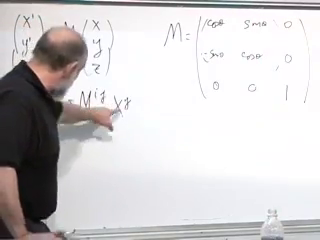
\includegraphics[width=0.82\textwidth]{lecture_05_figure_03.png}\caption{La rotación espacial expresada tanto mediante una ecuación matricial como en notación de índices.}\lectureframe{01:00:40}\end{figure}

\section{Matrices de Lorentz y composición de velocidades}

Para un movimiento a lo largo de \(x\), la transformación de Lorentz en unidades \(c=1\) es
\begin{align}
x'&=\gamma_v(x-vt), & y'&=y,\nonumber\\
z'&=z, & t'&=\gamma_v(t-vx),
\end{align}
donde
\begin{equation}
\gamma_v=\frac{1}{\sqrt{1-v^2}}.
\end{equation}
Con el orden de componentes \((x,y,z,t)\), queda
\begin{equation}
\begin{pmatrix}x'\\y'\\z'\\t'\end{pmatrix}
=
\begin{pmatrix}
\gamma_v&0&0&-\gamma_vv\\
0&1&0&0\\
0&0&1&0\\
-\gamma_vv&0&0&\gamma_v
\end{pmatrix}
\begin{pmatrix}x\\y\\z\\t\end{pmatrix}.
\label{eq:l5-lorentz-matrix}
\end{equation}

\begin{figure}[H]\centering
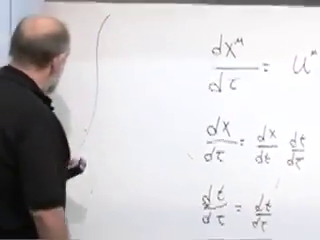
\includegraphics[width=0.82\textwidth]{lecture_05_figure_04.png}\caption{La matriz de Lorentz \(4\times4\). Solo se mezclan las componentes \(x\) y \(t\); \(y\) y \(z\) permanecen sin cambio.}\lectureframe{01:04:40}\end{figure}

La multiplicación de matrices permite responder ahora a una pregunta física. Supongamos que un observador se mueve con velocidad \(v\) respecto de nosotros y que un tercero se mueve con velocidad \(u\) respecto de ese observador, todos a lo largo del mismo eje. La cinemática newtoniana daría \(w=u+v\), lo que permitiría combinar dos velocidades de \(3c/4\) y obtener \(3c/2\). La relatividad debe dar una regla distinta.

La parte activa de la transformación de Lorentz es la matriz \(2\times2\)
\begin{equation}
B(v)=\gamma_v
\begin{pmatrix}1&-v\\-v&1\end{pmatrix}.
\end{equation}
Al componer las dos transformaciones se obtiene
\begin{align}
B(u)B(v)
&=\gamma_u\gamma_v
\begin{pmatrix}1&-u\\-u&1\end{pmatrix}
\begin{pmatrix}1&-v\\-v&1\end{pmatrix}\nonumber\\
&=\gamma_u\gamma_v
\begin{pmatrix}
1+uv&-(u+v)\\
-(u+v)&1+uv
\end{pmatrix}.
\label{eq:l5-composed-boost}
\end{align}
El cociente entre un elemento no diagonal y uno diagonal identifica la velocidad de la transformación resultante:
\begin{equation}
w=\frac{u+v}{1+uv}
\qquad(c=1).
\end{equation}
Al restablecer las dimensiones,
\begin{equation}
w=\frac{u+v}{1+uv/c^2}.
\label{eq:l5-velocity-addition}
\end{equation}

\begin{figure}[H]\centering
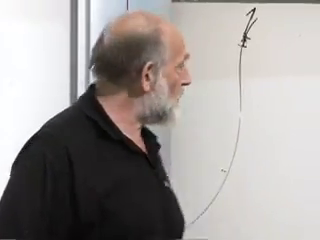
\includegraphics[width=0.82\textwidth]{lecture_05_figure_05.png}\caption{La matriz de la composición de dos transformaciones de Lorentz y la velocidad \(w=(u+v)/(1+uv)\) en unidades naturales.}\lectureframe{01:15:35}\end{figure}

Si \(u\) y \(v\) están ambas cerca de \(c\), el numerador se aproxima a \(2c\), mientras que el denominador se aproxima a \(2\); por tanto, \(w\) se aproxima a \(c\), no a \(2c\). En general, la ec.~\eqref{eq:l5-velocity-addition} transforma valores de entrada sublumínicos en un resultado sublumínico. La multiplicación de matrices ha incorporado automáticamente el límite de velocidad.

\section{Cuadrivectores y el fracaso de la velocidad ordinaria}

Un cuadrivector es cualquier objeto cuyas cuatro componentes se transforman bajo rotaciones y transformaciones de Lorentz del mismo modo que las coordenadas espaciotemporales. Si \(V^\mu\) es un cuadrivector, entonces, con nuestra convención de signos,
\begin{equation}
V_\mu=(-V^1,-V^2,-V^3,V^0),
\end{equation}
y su norma invariante es
\begin{equation}
V_\mu V^\mu=(V^0)^2-(V^1)^2-(V^2)^2-(V^3)^2.
\end{equation}
Para dos cuadrivectores \(V^\mu\) y \(W^\mu\), la contracción
\begin{equation}
W_\mu V^\mu
=W^0V^0-W^1V^1-W^2V^2-W^3V^3
\end{equation}
también es invariante. Las componentes cambian de un sistema de referencia a otro; la contracción no.

La velocidad ordinaria solo tiene tres componentes:
\begin{equation}
\mathbf v=\left(\frac{dx}{dt},\frac{dy}{dt},\frac{dz}{dt}\right).
\end{equation}
Añadir \(dt/dt=1\) no la convierte en un cuadrivector útil. La cuarta componente sería trivial y el objeto resultante no se transformaría linealmente bajo las transformaciones de Lorentz. El tiempo coordenado \(t\) cambia de un sistema de referencia a otro, así que derivar respecto de \(t\) arruina la ley de transformación deseada.

El tiempo propio resuelve el problema. A lo largo de una línea de universo, definamos
\begin{equation}
u^\mu=\frac{dX^\mu}{d\tau}.
\label{eq:l5-four-velocity}
\end{equation}
El diferencial \(dX^\mu\) es un cuadrivector y \(d\tau\) es invariante, de modo que su cociente también es un cuadrivector. El adjetivo ``propio'' alude al reloj que aparece en el denominador.

La regla de la cadena relaciona este objeto con la velocidad ordinaria:
\begin{equation}
\frac{dx}{d\tau}=\frac{dx}{dt}\frac{dt}{d\tau},
\end{equation}
y de igual modo para \(y\) y \(z\). De la ec.~\eqref{eq:l5-proper-time},
\begin{align}
\left(\frac{d\tau}{dt}\right)^2
&=1-\left(\frac{dx}{dt}\right)^2
    -\left(\frac{dy}{dt}\right)^2
    -\left(\frac{dz}{dt}\right)^2\nonumber\\
&=1-v^2
\qquad(c=1),
\end{align}
y, por tanto,
\begin{equation}
\frac{dt}{d\tau}=\gamma_v=\frac{1}{\sqrt{1-v^2}}.
\end{equation}
Las cuatro componentes son
\begin{equation}
u^i=\gamma_v v^i,
\qquad
u^0=\gamma_v
\qquad(c=1).
\label{eq:l5-four-velocity-components}
\end{equation}
A baja velocidad, \(u^i\simeq v^i\) y \(u^0\simeq1\). Cerca de la velocidad de la luz, \(\gamma_v\) crece sin límite y la velocidad propia difiere mucho de la velocidad ordinaria.

\begin{figure}[H]\centering
\includegraphics[width=0.82\textwidth]{lecture_05_figure_06.png}\caption{Las cuatro componentes de la velocidad propia expresadas en función de la velocidad ordinaria y del factor de Lorentz.}\lectureframe{01:34:40}\end{figure}

Al restablecer las unidades convencionales y usar \(X^0=ct\), se obtiene la forma estándar
\begin{equation}
U^\mu=(\gamma_v\mathbf v,\gamma_v c)
\end{equation}
con el orden espacial primero que se usa aquí. Su norma invariante es
\begin{equation}
U_\mu U^\mu=c^2.
\end{equation}
Así, todas las partículas masivas tienen una cuadrivelocidad de la misma magnitud invariante, aunque su velocidad espacial dependa del sistema de referencia.

\section{La tangente a una línea de universo}

La ec.~\eqref{eq:l5-four-velocity} tiene un modelo euclídeo familiar. A lo largo de una curva en el espacio tridimensional ordinario,
\begin{equation}
ds^2=dx^2+dy^2+dz^2.
\end{equation}
El desplazamiento diferencial \((dx,dy,dz)\) apunta a lo largo de la curva, pero no es un vector unitario. Al dividirlo por la longitud de arco se obtiene
\begin{equation}
\mathbf T=
\left(\frac{dx}{ds},\frac{dy}{ds},\frac{dz}{ds}\right),
\qquad
\mathbf T\cdot\mathbf T=1.
\end{equation}
La construcción relativista sigue la misma idea, pero usa el tiempo propio en lugar de la longitud de arco euclídea. El vector \(u^\mu=dX^\mu/d\tau\) es tangente a la línea de universo.

\begin{figure}[H]\centering
\includegraphics[width=0.82\textwidth]{lecture_05_figure_07.png}\caption{Construcción del vector tangente euclídeo: se divide el desplazamiento diferencial por el elemento de longitud de arco \(ds\). El tiempo propio cumple un papel análogo a lo largo de una línea de universo de tipo temporal.}\lectureframe{01:39:30}\end{figure}

\begin{classroomqa}\audiencequestion{Si \(c=1\), ¿son lo mismo el tiempo propio y la distancia propia?}\lecturerresponse{Tomar \(c=1\) pone el tiempo y la distancia en las mismas unidades; no elimina los signos menos de la geometría espaciotemporal. En la analogía euclídea, \(s\) es la distancia ordinaria medida a lo largo de una curva espacial. A lo largo de una línea de universo de tipo temporal, \(\tau\) es el tiempo transcurrido que mide un reloj. Las construcciones son análogas, pero las geometrías son distintas.}\end{classroomqa}

Al derivar una vez más se define la aceleración propia,
\begin{equation}
a^\mu=\frac{du^\mu}{d\tau}.
\end{equation}
Esta es la magnitud que debe sustituir a \(d^2\mathbf x/dt^2\) al formular la segunda ley de Newton de manera relativista. Como \(u_\mu u^\mu\) es constante,
\begin{equation}
\frac{d}{d\tau}(u_\mu u^\mu)=2u_\mu a^\mu=0,
\end{equation}
y, por tanto, la cuadraceleración es ortogonal a la cuadrivelocidad en la métrica de Minkowski.\editorialnote{La ortogonalidad se deduce directamente de la norma invariante y se incluye como siguiente consecuencia matemática de la definición.}

\section{Cuadrimomento y energía}

El momento es nuestro último ejemplo porque se conserva en colisiones y desintegraciones. La partícula tiene una masa intrínseca fija \(m\), llamada a menudo masa en reposo. No varía con la velocidad. El momento relativista es esa masa fija multiplicada por la cuadrivelocidad:
\begin{equation}
p^\mu=mu^\mu.
\label{eq:l5-four-momentum}
\end{equation}
En unidades \(c=1\),
\begin{equation}
p^i=\gamma_v m v^i,
\qquad
p^0=\gamma_v m.
\end{equation}
A velocidades bajas, \(\gamma_v\simeq1\), de modo que las componentes espaciales se reducen al momento newtoniano \(m\mathbf v\). A altas velocidades, crecen más rápidamente que \(m\mathbf v\).

La componente temporal es la energía. Con unidades convencionales y \(X^0=ct\),
\begin{equation}
P^\mu=(\mathbf p,E/c)
=(\gamma_v m\mathbf v,\gamma_v mc),
\end{equation}
y, por tanto,
\begin{equation}
E=\gamma_v mc^2
=mc^2\left(1-\frac{v^2}{c^2}\right)^{-1/2}.
\label{eq:l5-relativistic-energy}
\end{equation}

Para recuperar la mecánica ordinaria, tomemos
\(\epsilon=v^2/c^2\ll1\). El desarrollo binomial da
\begin{equation}
(1-\epsilon)^p=1-p\epsilon+O(\epsilon^2).
\end{equation}
Tomando \(p=-1/2\),
\begin{align}
E
&=mc^2\left(1-\frac{v^2}{c^2}\right)^{-1/2}\nonumber\\
&=mc^2\left[1+\frac12\frac{v^2}{c^2}
  +O\!\left(\frac{v^4}{c^4}\right)\right]\nonumber\\
&=mc^2+\frac12mv^2+O\!\left(\frac{mv^4}{c^2}\right).
\label{eq:l5-energy-expansion}
\end{align}

\begin{figure}[H]\centering
\includegraphics[width=0.82\textwidth]{lecture_05_figure_08.png}\caption{Desarrollo de la energía relativista a baja velocidad, que revela la energía en reposo y la energía cinética newtoniana.}\lectureframe{01:51:30}\end{figure}

El primer término, \(mc^2\), está presente incluso en reposo. En un problema newtoniano con un conjunto fijo de partículas y masas constantes, ese término suma la misma constante antes y después del movimiento, así que solo \(\tfrac12mv^2\) interviene en el balance habitual. La relatividad revela que esa constante descartada siempre fue energía física.

Por tanto, energía y momento no son leyes de conservación sin relación entre sí. Son las cuatro componentes de un único vector conservado. Una transformación de Lorentz los mezcla: lo que un observador llama energía contribuye en parte al momento de otro, y viceversa. Sin embargo, para un sistema aislado, el cuadrimomento total es el mismo antes y después de cualquier colisión o desintegración en todos los sistemas de referencia inerciales.

Este es el umbral de la mecánica relativista. Los siguientes pasos consisten en expresar la fuerza mediante la aceleración propia y comprender las ecuaciones de onda relativistas, en particular las que gobiernan el electromagnetismo y la luz.